\documentclass{standalone}
\usepackage{tikz}
\usetikzlibrary{patterns, positioning}

\begin{document}
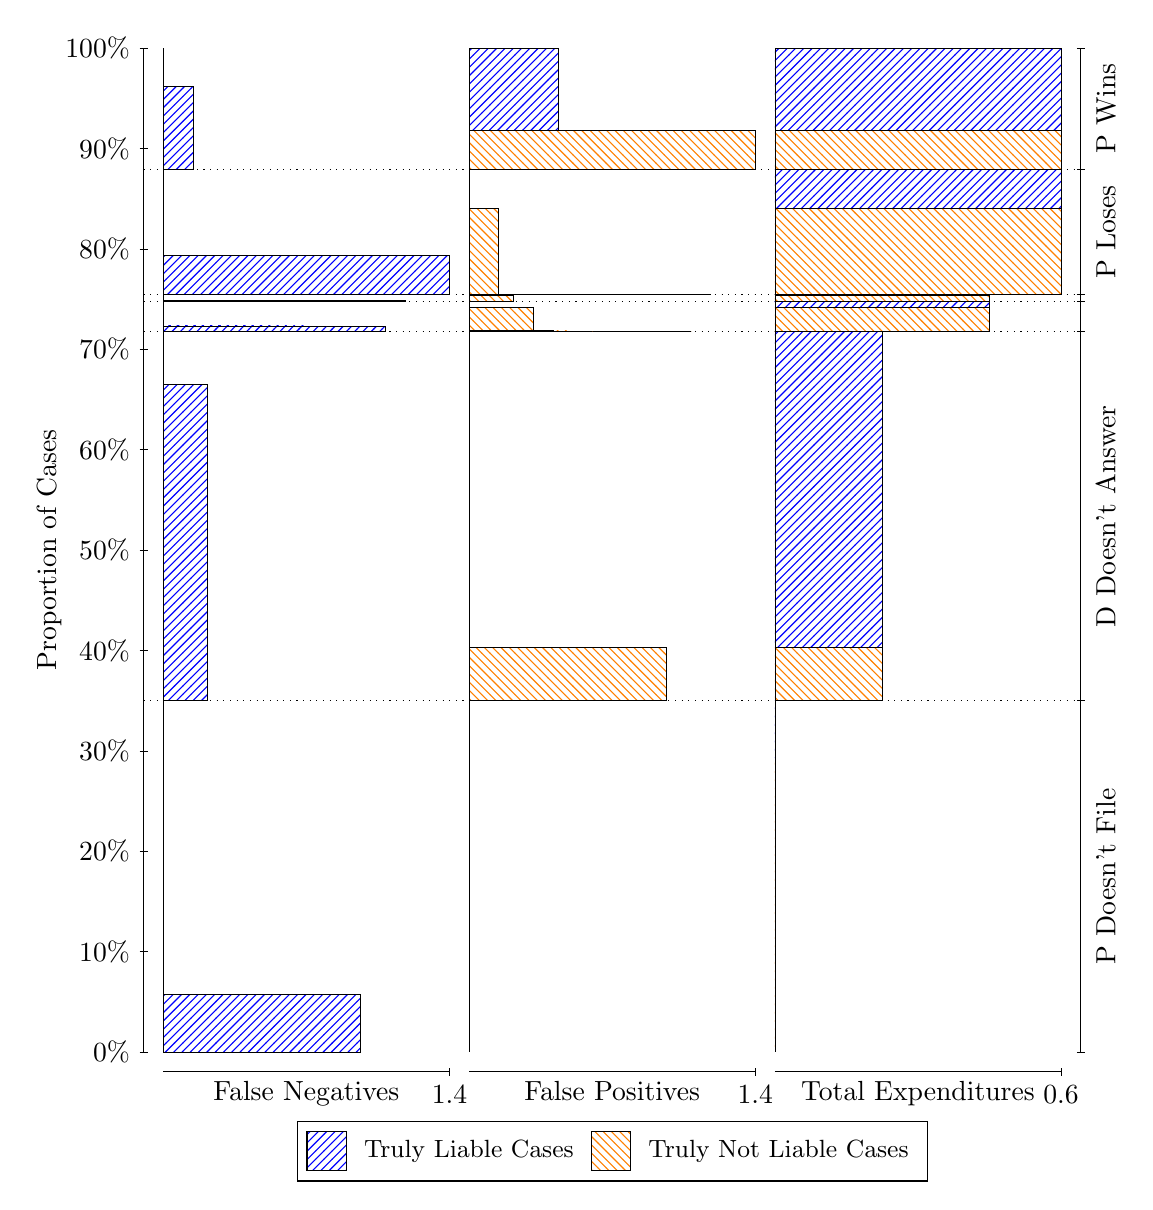
\begin{tikzpicture}
\draw[black, very thin] (1.5,1.75) -- (1.5,14.5);
\node[rotate=90, anchor=center] at (0.3, 8.125) {Proportion of Cases};
\draw[black, very thin] (1.45,1.75) -- (1.55,1.75);
\node[anchor=east] at (1.45, 1.75) {0\%};
\draw[black, very thin] (1.45,3.025) -- (1.55,3.025);
\node[anchor=east] at (1.45, 3.025) {10\%};
\draw[black, very thin] (1.45,4.3) -- (1.55,4.3);
\node[anchor=east] at (1.45, 4.3) {20\%};
\draw[black, very thin] (1.45,5.575) -- (1.55,5.575);
\node[anchor=east] at (1.45, 5.575) {30\%};
\draw[black, very thin] (1.45,6.85) -- (1.55,6.85);
\node[anchor=east] at (1.45, 6.85) {40\%};
\draw[black, very thin] (1.45,8.125) -- (1.55,8.125);
\node[anchor=east] at (1.45, 8.125) {50\%};
\draw[black, very thin] (1.45,9.4) -- (1.55,9.4);
\node[anchor=east] at (1.45, 9.4) {60\%};
\draw[black, very thin] (1.45,10.675) -- (1.55,10.675);
\node[anchor=east] at (1.45, 10.675) {70\%};
\draw[black, very thin] (1.45,11.95) -- (1.55,11.95);
\node[anchor=east] at (1.45, 11.95) {80\%};
\draw[black, very thin] (1.45,13.225) -- (1.55,13.225);
\node[anchor=east] at (1.45, 13.225) {90\%};
\draw[black, very thin] (1.45,14.5) -- (1.55,14.5);
\node[anchor=east] at (1.45, 14.5) {100\%};

\draw[black, very thin] (13.4,1.75) -- (13.4,14.5);
\draw[black, very thin] (13.35,1.75) -- (13.45,1.75);
\node[anchor=west] at (13.35, 1.75) {};
\draw[black, very thin] (13.35,6.2126) -- (13.45,6.2126);
\node[anchor=west] at (13.35, 6.2126) {};
\draw[black, very thin] (13.35,10.898) -- (13.45,10.898);
\node[anchor=west] at (13.35, 10.898) {};
\draw[black, very thin] (13.35,11.283) -- (13.45,11.283);
\node[anchor=west] at (13.35, 11.283) {};
\draw[black, very thin] (13.35,11.374) -- (13.45,11.374);
\node[anchor=west] at (13.35, 11.374) {};
\draw[black, very thin] (13.35,11.374) -- (13.45,11.374);
\node[anchor=west] at (13.35, 11.374) {};
\draw[black, very thin] (13.35,12.96) -- (13.45,12.96);
\node[anchor=west] at (13.35, 12.96) {};
\draw[black, very thin] (13.35,14.5) -- (13.45,14.5);
\node[anchor=west] at (13.35, 14.5) {};

\draw[black, very thin, pattern color=blue, pattern=north east lines] (1.75,1.75) rectangle (4.2557,2.4819);
\draw[black, very thin, pattern color=orange, pattern=north west lines] (1.75,2.4819) rectangle (1.75,6.2126);
\draw[black, very thin, pattern color=blue, pattern=north east lines] (1.75,6.2126) rectangle (2.3138,10.225);
\draw[black, very thin, pattern color=orange, pattern=north west lines] (1.75,10.225) rectangle (1.75,10.898);
\draw[black, very thin, pattern color=blue, pattern=north east lines] (1.75,10.898) rectangle (4.569,10.963);
\draw[black, very thin, pattern color=blue, pattern=north east lines] (1.75,10.963) rectangle (4.3184,10.964);
\draw[black, very thin, pattern color=blue, pattern=north east lines] (1.75,10.964) rectangle (4.0678,10.966);
\draw[black, very thin, pattern color=blue, pattern=north east lines] (1.75,10.966) rectangle (3.8172,10.966);
\draw[black, very thin, pattern color=blue, pattern=north east lines] (1.75,10.966) rectangle (3.5667,10.972);
\draw[black, very thin, pattern color=blue, pattern=north east lines] (1.75,10.972) rectangle (3.3161,10.972);
\draw[black, very thin, pattern color=blue, pattern=north east lines] (1.75,10.972) rectangle (3.0655,10.972);
\draw[black, very thin, pattern color=blue, pattern=north east lines] (1.75,10.972) rectangle (2.8149,10.972);
\draw[black, very thin, pattern color=blue, pattern=north east lines] (1.75,10.972) rectangle (2.5644,10.972);
\draw[black, very thin, pattern color=orange, pattern=north west lines] (1.75,10.972) rectangle (1.75,11.283);
\draw[black, very thin, pattern color=blue, pattern=north east lines] (1.75,11.283) rectangle (4.8195,11.299);
\draw[black, very thin, pattern color=orange, pattern=north west lines] (1.75,11.299) rectangle (1.75,11.374);
\draw[black, very thin, pattern color=blue, pattern=north east lines] (1.75,11.374) rectangle (2.3138,11.374);
\draw[black, very thin, pattern color=orange, pattern=north west lines] (1.75,11.374) rectangle (1.75,11.374);
\draw[black, very thin, pattern color=blue, pattern=north east lines] (1.75,11.374) rectangle (5.3833,11.865);
\draw[black, very thin, pattern color=orange, pattern=north west lines] (1.75,11.865) rectangle (1.75,12.96);
\draw[black, very thin, pattern color=blue, pattern=north east lines] (1.75,12.96) rectangle (2.1259,14.009);
\draw[black, very thin, pattern color=orange, pattern=north west lines] (1.75,14.009) rectangle (1.75,14.5);
\draw[black, very thin, pattern color=orange, pattern=north west lines] (5.6333,1.75) rectangle (5.6333,5.4807);
\draw[black, very thin, pattern color=blue, pattern=north east lines] (5.6333,5.4807) rectangle (5.6333,6.2126);
\draw[black, very thin, pattern color=orange, pattern=north west lines] (5.6333,6.2126) rectangle (8.1391,6.8857);
\draw[black, very thin, pattern color=blue, pattern=north east lines] (5.6333,6.8857) rectangle (5.6333,10.898);
\draw[black, very thin, pattern color=orange, pattern=north west lines] (5.6333,10.898) rectangle (8.4523,10.898);
\draw[black, very thin, pattern color=orange, pattern=north west lines] (5.6333,10.898) rectangle (8.2017,10.898);
\draw[black, very thin, pattern color=orange, pattern=north west lines] (5.6333,10.898) rectangle (7.9511,10.898);
\draw[black, very thin, pattern color=orange, pattern=north west lines] (5.6333,10.898) rectangle (7.7006,10.898);
\draw[black, very thin, pattern color=orange, pattern=north west lines] (5.6333,10.898) rectangle (7.45,10.905);
\draw[black, very thin, pattern color=orange, pattern=north west lines] (5.6333,10.905) rectangle (7.1994,10.905);
\draw[black, very thin, pattern color=orange, pattern=north west lines] (5.6333,10.905) rectangle (6.9489,10.907);
\draw[black, very thin, pattern color=orange, pattern=north west lines] (5.6333,10.907) rectangle (6.6983,10.91);
\draw[black, very thin, pattern color=orange, pattern=north west lines] (5.6333,10.91) rectangle (6.4477,11.209);
\draw[black, very thin, pattern color=blue, pattern=north east lines] (5.6333,11.209) rectangle (5.9466,11.209);
\draw[black, very thin, pattern color=blue, pattern=north east lines] (5.6333,11.209) rectangle (5.696,11.209);
\draw[black, very thin, pattern color=blue, pattern=north east lines] (5.6333,11.209) rectangle (5.6333,11.283);
\draw[black, very thin, pattern color=orange, pattern=north west lines] (5.6333,11.283) rectangle (6.1971,11.357);
\draw[black, very thin, pattern color=blue, pattern=north east lines] (5.6333,11.357) rectangle (5.6333,11.374);
\draw[black, very thin, pattern color=orange, pattern=north west lines] (5.6333,11.374) rectangle (8.7029,11.374);
\draw[black, very thin, pattern color=blue, pattern=north east lines] (5.6333,11.374) rectangle (6.1971,11.374);
\draw[black, very thin, pattern color=orange, pattern=north west lines] (5.6333,11.374) rectangle (6.0092,12.468);
\draw[black, very thin, pattern color=blue, pattern=north east lines] (5.6333,12.468) rectangle (5.6333,12.96);
\draw[black, very thin, pattern color=orange, pattern=north west lines] (5.6333,12.96) rectangle (9.2667,13.451);
\draw[black, very thin, pattern color=blue, pattern=north east lines] (5.6333,13.451) rectangle (6.7609,14.5);
\draw[black, very thin, pattern color=orange, pattern=north west lines] (9.5167,1.75) rectangle (9.5167,5.4807);
\draw[black, very thin, pattern color=blue, pattern=north east lines] (9.5167,5.4807) rectangle (9.5167,6.2126);
\draw[black, very thin, pattern color=orange, pattern=north west lines] (9.5167,6.2126) rectangle (10.879,6.8857);
\draw[black, very thin, pattern color=blue, pattern=north east lines] (9.5167,6.8857) rectangle (10.879,10.898);
\draw[black, very thin, pattern color=orange, pattern=north west lines] (9.5167,10.898) rectangle (12.242,10.898);
\draw[black, very thin, pattern color=blue, pattern=north east lines] (9.5167,10.898) rectangle (12.242,10.898);
\draw[black, very thin, pattern color=orange, pattern=north west lines] (9.5167,10.898) rectangle (12.242,11.207);
\draw[black, very thin, pattern color=blue, pattern=north east lines] (9.5167,11.207) rectangle (12.242,11.279);
\draw[black, very thin, pattern color=orange, pattern=north west lines] (9.5167,11.279) rectangle (12.242,11.282);
\draw[black, very thin, pattern color=blue, pattern=north east lines] (9.5167,11.282) rectangle (12.242,11.283);
\draw[black, very thin, pattern color=orange, pattern=north west lines] (9.5167,11.283) rectangle (12.242,11.283);
\draw[black, very thin, pattern color=blue, pattern=north east lines] (9.5167,11.283) rectangle (12.242,11.283);
\draw[black, very thin, pattern color=orange, pattern=north west lines] (9.5167,11.283) rectangle (12.242,11.357);
\draw[black, very thin, pattern color=blue, pattern=north east lines] (9.5167,11.357) rectangle (12.242,11.374);
\draw[black, very thin, pattern color=orange, pattern=north west lines] (9.5167,11.374) rectangle (12.242,11.374);
\draw[black, very thin, pattern color=blue, pattern=north east lines] (9.5167,11.374) rectangle (12.242,11.374);
\draw[black, very thin, pattern color=orange, pattern=north west lines] (9.5167,11.374) rectangle (13.15,12.468);
\draw[black, very thin, pattern color=blue, pattern=north east lines] (9.5167,12.468) rectangle (13.15,12.96);
\draw[black, very thin, pattern color=orange, pattern=north west lines] (9.5167,12.96) rectangle (13.15,13.451);
\draw[black, very thin, pattern color=blue, pattern=north east lines] (9.5167,13.451) rectangle (13.15,14.5);
\draw[black, dotted] (1.5,6.2126) -- (13.4,6.2126);
\draw[black, dotted] (1.5,10.898) -- (13.4,10.898);
\draw[black, dotted] (1.5,11.283) -- (13.4,11.283);
\draw[black, dotted] (1.5,11.374) -- (13.4,11.374);
\draw[black, dotted] (1.5,11.374) -- (13.4,11.374);
\draw[black, dotted] (1.5,12.96) -- (13.4,12.96);
\draw[black, very thin] (1.75,1.5) -- (5.3833,1.5);
\node[anchor=north] at (3.5667, 1.5) {False Negatives};
\draw[black, very thin] (5.3833,1.45) -- (5.3833,1.55);
\node[anchor=north] at (5.3833, 1.45) {1.4};

\draw[black, very thin] (5.6333,1.5) -- (9.2667,1.5);
\node[anchor=north] at (7.45, 1.5) {False Positives};
\draw[black, very thin] (9.2667,1.45) -- (9.2667,1.55);
\node[anchor=north] at (9.2667, 1.45) {1.4};

\draw[black, very thin] (9.5167,1.5) -- (13.15,1.5);
\node[anchor=north] at (11.333, 1.5) {Total Expenditures};
\draw[black, very thin] (13.15,1.45) -- (13.15,1.55);
\node[anchor=north] at (13.15, 1.45) {0.6};

\node[black, centered, rotate=90] at (13.72, 3.9813) {P Doesn't File};
\node[black, centered, rotate=90] at (13.72, 8.5554) {D Doesn't Answer};



\node[black, centered, rotate=90] at (13.72, 12.167) {P Loses};
\node[black, centered, rotate=90] at (13.72, 13.73) {P Wins};

\draw (7.449999999999999,1.5) node[draw=none] (baseCoordinate) {};
\begin{scope}[align=center]
        \matrix[scale=0.5, draw=black, below=0.5cm of baseCoordinate, nodes={draw}, column sep=0.1cm]{
            \node[rectangle, draw, minimum width=0.5cm, minimum height=0.5cm, pattern=north east lines, pattern color=blue] {}; &
            \node[draw=none, font=\small] (B) {Truly Liable Cases}; &
            \node[rectangle, draw, minimum width=0.5cm, minimum height=0.5cm, pattern=north west lines, pattern color=orange] {}; &
            \node[draw=none, font=\small] (B) {Truly Not Liable Cases}; \\
            };
\end{scope}

\end{tikzpicture}
\end{document}